\documentclass{article}
\usepackage{arxiv}

\usepackage[utf8]{inputenc}
\usepackage[english, russian]{babel}
\usepackage[T1]{fontenc}
\usepackage{url}
\usepackage{booktabs}
\usepackage{amsfonts}
\usepackage{bbm}
\usepackage{nicefrac}
\usepackage{microtype}
\usepackage{lipsum}
\usepackage{graphicx}
\usepackage{natbib}
\usepackage{doi}



\title{Бэггинг над MARS со случайными поворотами признаков}

\author{ David S.~Hippocampus\thanks{Use footnote for providing further
		information about author (webpage, alternative
		address)---\emph{not} for acknowledging funding agencies.} \\
	Department of Computer Science\\
	Cranberry-Lemon University\\
	Pittsburgh, PA 15213 \\
	\texttt{hippo@cs.cranberry-lemon.edu} \\
	%% examples of more authors
	\And
	Elias D.~Striatum \\
	Department of Electrical Engineering\\
	Mount-Sheikh University\\
	Santa Narimana, Levand \\
	\texttt{stariate@ee.mount-sheikh.edu} \\
	%% \AND
	%% Coauthor \\
	%% Affiliation \\
	%% Address \\
	%% \texttt{email} \\
	%% \And
	%% Coauthor \\
	%% Affiliation \\
	%% Address \\
	%% \texttt{email} \\
	%% \And
	%% Coauthor \\
	%% Affiliation \\
	%% Address \\
	%% \texttt{email} \\
}
\date{}

\renewcommand{\shorttitle}{\textit{arXiv} Template}

%%% Add PDF metadata to help others organize their library
%%% Once the PDF is generated, you can check the metadata with
%%% $ pdfinfo template.pdf
\hypersetup{
pdftitle={Бэггинг над MARS со случайными поворотами признаков},
pdfsubject={q-bio.NC, q-bio.QM},
pdfauthor={David S.~Hippocampus, Elias D.~Striatum},
pdfkeywords={First keyword, Second keyword, More},
}

\begin{document}
\maketitle


\begin{abstract}
Алгоритм multivariate adaptive regression splines (MARS) обеспечивает гибкий
метод статистического моделирования, который использует прямой и обратный проходы, где происходит подбор порогов и переменных, для определения комбинации
базовых функций, которые наилучшим образом приближают исходные данные.
В области оптимизации MARS успешно использовался для оценки неизвестных функций в стохастическом динамическом программировании, стохастическом программировании и в других направлениях. MARS потенциально может быть полезен во многих реальных задачах оптимизации, где необходимо оценить целевую функцию на основе наблюдаемых данных. Однако использование MARS в ансамбле позволяет добиться даже большего качества на данных. Использование случайных ортогональных преобразований в ансамбле может сделать алгоритм менее чувствительным к расположению признаков в пространстве. Таким образом, получается найти более оптимальное приближение целевой функции в задаче регрессии.
\end{abstract}


\keywords{MARS \and Сплайны \and Регрессия}

\section{Introduction}
%\lipsum[2]
%\lipsum[3]
В качестве популярного метода непараметрической регрессии алгоритм 
многомерных адаптивных регрессионных сплайнов (MARS) был впервые представлен Джеромом Фридманом в 1991 г. \cite{friedman1991multivariate}. Благодаря своей гибкости и точности MARS использовался во многих исследованиях, где возникает классическая для машинного обучения задача регрессии, включая прогнозирование спроса на энергию, необходимую для транспортировки (M.A. Sahraei, H. Duman, M.Y. Çodur et al, 2021) \cite{sahraei2021prediction}, анализ реакций роста, связанных с макропитательными веществами (M Akin et al, 2020) \cite{akin2020analysis}, построение системы принятия решений по борьбе с загрязнением озоном (Yang, Chen, Chang, Sattler, \& Wen, 2009) \cite{yang2009decision}, оценку подверженности овражной эрозии (Conoscenti, Agnesi, Cama, Caraballo-Arias, \& Rotigliano, 2018) \cite{conoscenti2018assessment}, оценку тепловой нагрузки в зданиях (Roy, Roy, \& Balas, 2018) \cite{roy2018estimating}, моделирование суточной концентрации растворенного кислорода (Heddam \& Kisi, 2018) \cite{heddam2018modelling} и др.
Также MARS используется и в медицинских целях, например, для выявления влияния пола на факторы, оказывающих воздействие на нарушения опорно-двигательного аппарата плеч, шеи и верхних конечностей
(Serrano, Sanchez, Lasheras, Iglesias-Rodríguez, \& Valverde, 2020) \cite{serrano2020identification}.

С момента появления классического алгоритма MARS~\cite{friedman1991multivariate} уже было произведено множество исследований, направленных на улучшение точности предсказания в задаче регрессии и ускорение обучения модели. Одними из первых стали модели с полиномиальными сплайнами \cite{stone1997polynomial}, в которой удаление базисной функции из алгоритма влекло за собой последующее удаление всех произведенных от нее элементов, и баесовская модификация MARS~\cite{denison1998bayesian}, где использовались марковские цепи и метод Монте-Карло.
Еще одним ответвлением стал CMARS~\cite{weber2012cmars}, использующий непрерывные методы оптимизации и регуляризации. 

Чтобы улучшить точность предсказаний алгоритма MARS и время обучения, были испробованы различные подходы. Например, ранее был предложен способ быстрой оптимизации узлов с использованием метода восхождения к вершине, где перебор порогов начинается с точки, на которой был достигнут максимум на предыдущем шаге (Xinglong Ju, Victoria C.P. Chen, 2021) \cite{ju2021fast}. Также в MARS можно использовать B-сплайны, что показало свою эффективность в решении задачи регрессии (Sergey Bakin, Markus Hegland \& Michael R. Osborne, 2000) \cite{bakin2000parallel}, либо другие улучшения, как Robust MARS (Ozmen \& Weber, 2014) \cite{ozmen2011rcmars}, который лучше справляется с менее надежными данными. Существую и другие подходы, расширяющие применение MARS, например, выпуклый вариант MARS, подходящий для решения специфических типов задач (Martinez, Diana L., et al, 2015)\cite{martinez2015convex}

В данной работе предлагается использовать бэггинг над MARS (Реализация PyEarth\footnote{\url{https://github.com/scikit-learn-contrib/py-earth}}), а так же использовать модификацию - случайный поворот признаков, на которых в последствии будет обучаться алгоритм. Предыдущие подходы не учитывали случай, предполагающий, что базисная функция может функционально зависеть от, например, некоторой линейной комбинации признаков. В таком случае целевая переменная не представима в виде базисных функций, которые предлагают строить другие подходы. Однако использование ансамбля моделей, где каждая модель использует свое собственное признаковое пространство, позволяет нивелировать данную проблему.

\section{Постановка задачи}
\label{sec:headings}

%\lipsum[4] See Section \ref{sec:headings}.
В задачах регрессии целевая переменная $y$ представляется в виде функции от $p$ переменных с некоторым шумом $\varepsilon$: $$y=f(x^1, x^2, ..., x^p) + \varepsilon,$$ где f неизвестная функция, и $\mathbbm{E}\varepsilon = 0$.

По рассматриваемому набору данных $D = \{x_i, y_i\}_{i=1}^{N}$, функция $f(x^1, x^2, ..., x^p)$ аппроксимируется некоторой функцией $g(x^1, x^2, ..., x^p)$. Качество аппроксимации оценивается с помощью среднего квадрата ошибки (MSE):
$$MSE(D) = \frac{1}{N}\sum_{k=1}^{N} (g(x_k) - y_k)^2$$
либо схожей величины $RMSE(D) = \sqrt{MSE(D)}$.
Считается, что модель с меньшим значением среднего квадрата ошибки лучше соответствует
данным.

В данной работе функция $g(x)$ строилась согласно алгоритму MARS (Multivariate Adaptive Regression Splines) \cite{friedman1991multivariate}, который аппроксимирует исходную функцию $f$ в виде:
$$h(x) = \sum_{m=0}^{M} a_m \cdot B_m(x),$$ где $B_m(x) = \prod_{k=1}^{K_m} b_{k,m}.$
$b_{k,m}$ - базисная функция от одной переменной, которая имеет вид либо $max\{+(x-t),~0\}$, либо $max\{-(x-t), 0\}.$

\subsection{Headings: second level}
\lipsum[5]
\begin{equation}
	\xi _{ij}(t)=P(x_{t}=i,x_{t+1}=j|y,v,w;\theta)= {\frac {\alpha _{i}(t)a^{w_t}_{ij}\beta _{j}(t+1)b^{v_{t+1}}_{j}(y_{t+1})}{\sum _{i=1}^{N} \sum _{j=1}^{N} \alpha _{i}(t)a^{w_t}_{ij}\beta _{j}(t+1)b^{v_{t+1}}_{j}(y_{t+1})}}
\end{equation}

\subsubsection{Headings: third level}
\lipsum[6]

\paragraph{Paragraph}
\lipsum[7]



\section{Examples of citations, figures, tables, references}
\label{sec:others}

\subsection{Citations}
Citations use \verb+natbib+. The documentation may be found at
\begin{center}
	\url{http://mirrors.ctan.org/macros/latex/contrib/natbib/natnotes.pdf}
\end{center}

Here is an example usage of the two main commands (\verb+citet+ and \verb+citep+): Some people thought a thing \citep{kour2014real, hadash2018estimate} but other people thought something else \citep{kour2014fast}. Many people have speculated that if we knew exactly why \citet{kour2014fast} thought this\dots

\subsection{Figures}
\lipsum[10]
See Figure \ref{fig:fig1}. Here is how you add footnotes. \footnote{Sample of the first footnote.}
\lipsum[11]

\begin{figure}
	\centering
	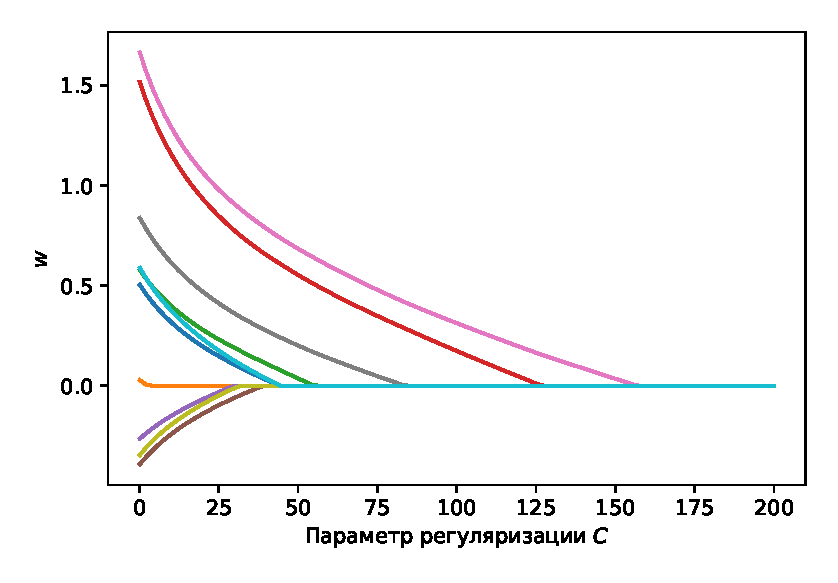
\includegraphics[width=0.5\textwidth]{../figures/log_reg_cs_exp.eps}
	\caption{Sample figure caption.}
	\label{fig:fig1}
\end{figure}

\subsection{Tables}
See awesome Table~\ref{tab:table}.

The documentation for \verb+booktabs+ (`Publication quality tables in LaTeX') is available from:
\begin{center}
	\url{https://www.ctan.org/pkg/booktabs}
\end{center}


\begin{table}
	\caption{Sample table title}
	\centering
	\begin{tabular}{lll}
		\toprule
		\multicolumn{2}{c}{Part}                   \\
		\cmidrule(r){1-2}
		Name     & Description     & Size ($\mu$m) \\
		\midrule
		Dendrite & Input terminal  & $\sim$100     \\
		Axon     & Output terminal & $\sim$10      \\
		Soma     & Cell body       & up to $10^6$  \\
		\bottomrule
	\end{tabular}
	\label{tab:table}
\end{table}

\subsection{Lists}
\begin{itemize}
	\item Lorem ipsum dolor sit amet
	\item consectetur adipiscing elit.
	\item Aliquam dignissim blandit est, in dictum tortor gravida eget. In ac rutrum magna.
\end{itemize}


\bibliographystyle{plain}
\bibliography{references}

\end{document}
